%%%%%%%%%%%%%%%%%%%%%%%%%%%%%%%%%%%%%%%%%%%%%%%
%%% DISCLAIMER: The original template for this
%%% file can be found at:
%%%
%%% https://www.overleaf.com/latex/templates/report-template-stima-laborations-overleaf-v1-dot-0/jtctxkqjnjdz
%%%
%%% Template for lab reports for CS341 @ IITB
%%%%%%%%%%%%%%%%%%%%%%%%%%%%%%%%%%%%%%%%%%%%%%%

%%%%%%%%%%%%%%%%%%%%%%%%%%%%%% Sets the document class for the document
% Openany is added to remove the book style of starting every new chapter on an odd page (not needed for reports)
\documentclass[11pt, swedish, openany]{book}

%%%%%%%%%%%%%%%%%%%%%%%%%%%%%% Loading packages that alter the style
\usepackage[]{graphicx}
\usepackage[]{color}
\usepackage{alltt}
\usepackage[T1]{fontenc}
\usepackage[utf8]{inputenc}
\usepackage{float}
\usepackage{multirow}
\usepackage{tablefootnote}
\usepackage{wrapfig}
\usepackage{amsmath}
\usepackage{placeins}
\usepackage{float}
\usepackage{subcaption}
\usepackage{makecell}
\usepackage{fancyvrb}

\setcounter{secnumdepth}{3}
\setcounter{tocdepth}{3}
\setlength{\parskip}{\smallskipamount}
\setlength{\parindent}{0pt}

% Set page margins
\usepackage[top=100pt, bottom=100pt, left=60pt, right=60pt]{geometry}

% Package used for placeholder text
\usepackage{lipsum}

% Prevents LaTeX from filling out a page to the bottom
\raggedbottom

% Adding both languages, Swedish and English, so they can be used intermittently in for example abstracts.
\usepackage[swedish, english]{babel}

% All page numbers positioned at the bottom of the page
\usepackage{fancyhdr}
\fancyhf{} % clear all header and footers
\fancyfoot[C]{\thepage}
\renewcommand{\headrulewidth}{0pt} % remove the header rule
\pagestyle{fancy}

% Changes the style of chapter headings
\usepackage{titlesec}
\titleformat{\chapter}{\normalfont\LARGE\bfseries}{\thechapter.}{1em}{}
% Change distance between chapter header and text
\titlespacing{\chapter}{0pt}{50pt}{2\baselineskip}

% Adds table captions above the table per default
\usepackage{float}
\floatstyle{plaintop}
\restylefloat{table}

% Adds space between caption and table
\usepackage[tableposition=top]{caption}

% Adds hyperlinks to references and ToC
\usepackage{hyperref}
\hypersetup{hidelinks, linkcolor = blue} % Changes the link color to black and hides the hideous red border that usually is created

% If multiple images are to be added, a folder (path) with all the images can be added here
\graphicspath{{images/}}

% Separates the first part of the report/thesis in Roman numerals
\frontmatter


%%%%%%%%%%%%%%%%%%%%%%%%%%%%%% Starts the document
\begin{document}

%%% Selects the language to be used for the first couple of pages
\selectlanguage{english}

%%%%% Adds the title page
\begin{titlepage}
    \clearpage\thispagestyle{empty}
    \centering
    \vspace{2cm}

    % Titles
    {\large CS341: Computer Architecture Lab\par}
    \vspace{4cm}
    {\Huge \textbf{Lab 5: Hacking ChampSim}} \\
    \vspace{0.2cm}
    {\huge \textbf{Report} \par}
    \vspace{4cm}
    % ========================================================
    % If this is a team-based project, add in your team-name,
    % team members along with roll numbers.
    %
    % If this is an individual project, remove the line
    % corresponding to team name and the remaining members
    % ========================================================
    {\normalsize {\large \textbf{Team ARCHimedes}}\\
        Vibhav Aggarwal (\texttt{190050128}) \\
        Adithya Bhaskar (\texttt{190050005}) \\
        Devansh Jain (\texttt{190100044}) \\
        Harshit Varma (\texttt{190100055}) \\
        Harshit Gupta (\texttt{190050048})
        %
        % Add more team members if there are any
        %
        \par}
    \vspace{2cm}
    \vfill

    
\includegraphics[scale=0.30]{iitb_logo/iitb_logo.eps}

    \vspace{0.5cm}

    % Information about the University
    {\normalsize
        Department of Computer Science and Engineering \\
        Indian Institute of Technology Bombay  \par}

    % Set the date
    {\normalsize 2021-2022 \par}
    \vspace{2cm}

    \pagebreak

\end{titlepage}

% Adds a table of contents
\tableofcontents{}

\clearpage

% Uncomment the following three rows for a table of figures and/or tables as they are not needed for lab reports
% \listoffigures
% \clearpage
% \listoftables

\mainmatter

%%%%%%%%%%%%%%%%%%%%%%%%%%%%%%%%%%%%%%%%%%%%%%%%
%% Abstract
%%%%%%%%%%%%%%%%%%%%%%%%%%%%%%%%%%%%%%%%%%%%%%%%
\chapter*{\centerline{Abstract}}
Summarize the objective of the lab, what experiments you have conducted, what were the results that you have obtained in a clear and concise manner. Numbers matter, not just words only, for ex. \emph{very high}, \emph{slow} etc.


%%%%%%%%%%%%%%%%%%%%%%%%%%%%%%%%%%%%%%%%%%%%%%%%
%% Understanding the problem statement
%%%%%%%%%%%%%%%%%%%%%%%%%%%%%%%%%%%%%%%%%%%%%%%%
\chapter{Understanding the problem statement}

\section{Summary of MadCache}
MadCache is an adaptive insertion policy that uses the Program Counter (PC) behavior history to determine the appropriate insertion policy for the Last Level Cache (LLC). It decides whether a miss should be saved in the cache or bypassed to the L2 Cache (L2C). In other words, choose between LRU (Least Recently Used) mode and bypassing mode.
The underlying assumption is that if a particular PC in a program exhibits streaming behavior, it will likely continue to do so, and should be prevented from flushing out other useful entries in the LLC.
While a PC may exhibit streaming behavior for one portion of the program, it is possible it changes its behavior later on. For such a case, thrashing protection must be enabled to allow a PC to get out of bypass mode.
Bypassing Bimodal Insertion Policy is the Bypassing version of BIP, which bypasses the majority of the incoming cachelines anticipating streaming activity and inserts a few lines to the LLC. \\

MadCache uses four structures to adapt the insertion policy of the LLC.
A 10-bit counter whose MSB is used to determine the default insertion policy. If the MSB is 1, then the default policy is BBIP.
A subset of the cache sets are called trackers sets, and the behavior of PCs accessing this set determines the counter value through set dueling.
The rest of the sets, in fact, the majority of the cache are called follower sets, and they simply adhere to the default insertion policy.
A lookup table referred to as the ``PC-predictor’’ is used to keep track of the history of PCs that have accessed the tracker sets. It has 1024 entries of 3 columns - (Default policy at the time of the entry of this PC, PC), a 6-bit counter whose MSB determines the behavior for this PC, and the number of entries associated with the PC. \\

At the start, the PC-predictor and the cache are empty, and the counter is set to 511, i.e., just below the threshold for BBIP.
After an initial LLC miss for a cacheline in the tracker sets, the invoking PC would be added to the PC-predictor. The counter for the entry is set to 63, i.e., just below the threshold of BBIP. The cacheline would be added to the LLC. The cacheline (in the tracker set) would also store the index to the table and a reuse bit to reward or penalize the tracked PC entry.
If the cacheline is accessed again, the counter for the PC entry would be decremented (in favor of LRU). However, if the cacheline is evicted without being reused, then the counter would be incremented (in favor of BBIP).
Entries from the PC-predictor are evicted when the number of cachelines brought in by the PC entry falls to zero.

A more detailed explanation of the MadCache policy is given in \autoref{LLC Bypassing}. \\

MadCache performs faster than both LRU and DIP, resulting in a 4.5\% speedup over LRU.


\section{Understanding ChampSim code}
\begin{itemize}
    \item The \texttt{handle\_read} function is responsible for reading a query from the read queue and processing it.\\
          A read hit means that the line requested is present in the cache. So, the data is read from the cache itself. Following are the things that are done on a hit:
          \begin{itemize}
              \item Get a read request from the read queue \texttt{RQ}. If no read request, return.
              \item Get the set and the way corresponding to the request address. For a hit, there must be a way with same address as the requested one. This is done using the \texttt{get\_set} and \texttt{check\_hit} functions.
              \item Read the data and update it in the packet that we got from the read queue.
              \item If it is a load request, update the prefetcher using the prefetcher\_operate functions
              \item Update the replacement policy using the update\_replacement\_policy functions. aThis corresponds to bringing the accessed block to MRU position in the LRU scheme.
              \item Mark the entry in the MSHR of higher level as completed and add the data to it. This is done using the \texttt{return\_data} function for the correct upper level cache. Notice that for L1D, L1I, ITLB and DTLB do not have a higher level cache. Instead, they put the data in the PROCESSING queue.
              \item Update the statistics like number of hits and number of accesses.
          \end{itemize}
    \item A read miss means that the line requested is not present in the cache. In such a case, we do the following:(skipping over getting the query and detecting a miss as it is same as hit)
          \begin{itemize}
              \item First we need to check if there is a read request for the same address already in MSHR or not. If there is we can merge the requests. This is done using the \texttt{check\_mshr} function.
                    \begin{itemize}
                        \item If the address is not in MSHR, we need to add a new entry in MSHR and read queue of the lower level. Adding to MSHR is done using \texttt{add\_mshr} function. Adding to the lower level's read queue is done using \texttt{lower\_level->add\_rq} function. (This function also checks if the request can be served from the write queue or not and adds the request to read queue only if it can't be done)\\
                              During the above operations, we need to ensure that we don't exceed the size of MSHR's and the queues. If this is the case, we must stall.
                        \item If the address is in MSHR, we need to merge the requests.\\
                              There is a member set named  \texttt{index\_depend\_on\_me} (different sets for load, store and instruction) in teh \texttt{PACKET} class. This set stores the index of all the requests depending on it. Merging indices amounts to joining the correct sets from request to MSHR entry and insert the index of request to the MSHR entry.
                    \end{itemize}
              \item Update statistics like number of misses, number of MSHR entries merged etc.
          \end{itemize}
    \item The \texttt{handle\_fill} function is responsible for processing the completed requests in MSHR and put the data in correct position in the cache. Any function serving a read request uses \texttt{return\_data} which only adds the data to the MSHR entry for that address. But we need the data in cache and not in MSHR. The work of getting the data from MSHR and writing to cache is done by \texttt{handle\_fill}. That is why it needs to read (completed) request from MSHR.
    \item The lower\_level, upper\_level data members are declared in teh MEMORY class. Since CACHE class inherits from MEMORY, it also has these data members. They are assigned in \texttt{main.cc} in the \texttt{main} function for all the caches.\\
          These are arrays which store pointer to the next lower or next higher cache in the memory hierarchy (if they do not exist, then set to NULL). Since we have different instruction and data cache at L1, we need 2 different upper\_level cache array, one for data and one for instruction. So, for example for L2 cache, the values are:\\
          ooo\_cpu[i].upper\_level\_icache = ooo\_cpu[i].L1I\\
          ooo\_cpu[i].upper\_level\_dcache = ooo\_cpu[i].L1D\\
          ooo\_cpu[i].lower\_level = uncore.LLC\\
          Notice that L1D, L1I, L2 and the TLBs are CPU specific while the LLC and DRAM are shared.
    \item The \texttt{return\_data} function is responsible for adding the data in an MSHR entry and marking it as completed. It takes a PACKET object as argument which stores the address and data. The basic workflow is:
          \begin{itemize}
              \item Find the MSHR entry with the same address as the one mentioned in the given packet. This is done using \texttt{check\_mshr} function. If it does not exist, return error
              \item Mark the MSHR entry as completed(setting returned to COMPLETED) and add the data and metadata to the MSHR entry.
              \item Update the metrics like number of requests returned and latency
              \item Update \texttt{next\_fill\_index} using \texttt{update\_fill\_cycle} function. This index is the index from which \texttt{read\_fill} reads the request to be written in the cache.
          \end{itemize}
\end{itemize}



%%%%%%%%%%%%%%%%%%%%%%%%%%%%%%%%%%%%%%%%%%%%%%%%
%% LLC Bypassing
%%%%%%%%%%%%%%%%%%%%%%%%%%%%%%%%%%%%%%%%%%%%%%%%
\chapter{LLC Bypassing}
\label{LLC Bypassing}

\section{Implementation}
The relevant output files are in their respective directories, as required by the problem statement. We proceed to describe our implementation of MadCache. We begin with the description of the \textit{predictor} structure. Refer to the illustration below.
\begin{figure}[H]
    \centering
    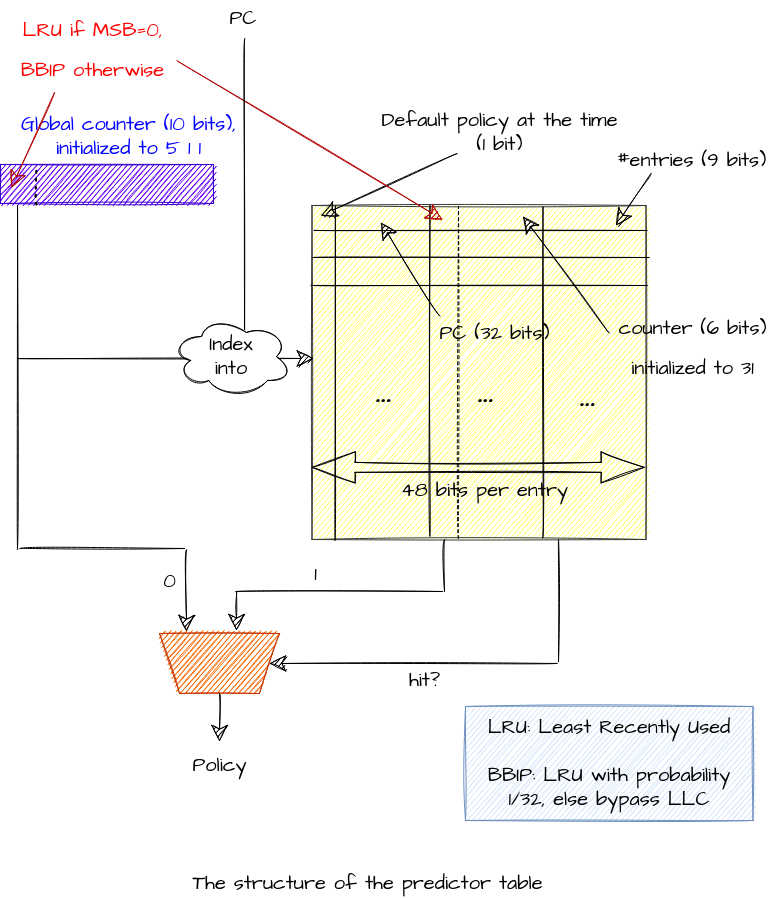
\includegraphics[width=0.55\linewidth]{images/predictor.png}
\end{figure}
The predictor consists of a global 10-bit counter (which determines the global default policy, initialized to 0111111111 or 511) and a set of entries each with their counters, which determines PC-specific policies. In particular, if the MSB of the global counter is 0, the default policy is LRU; else, it is to use BBIP. Here, BBIP uses LRU 1/32-th of the time and bypasses otherwise. Each entry contains:
\begin{itemize}
    \item \textbf{Default policy and PC:} This consists of the PC used when fetching the cacheline which led to the creation of this entry, and the default policy at the time.
    \item \textbf{Counter:} A 6-bit counter governing the PC-specific policy, of 6 bits.
    \item \textbf{Number of entries:} This field tells us how many cachelines currently use this entry (0 if none).
\end{itemize}
Next we describe how we use this predictor to decide what to do with newly fetched cachelines from DRAM to the LLC. Refer to the flowchart below.
\begin{figure}[H]
    \centering
    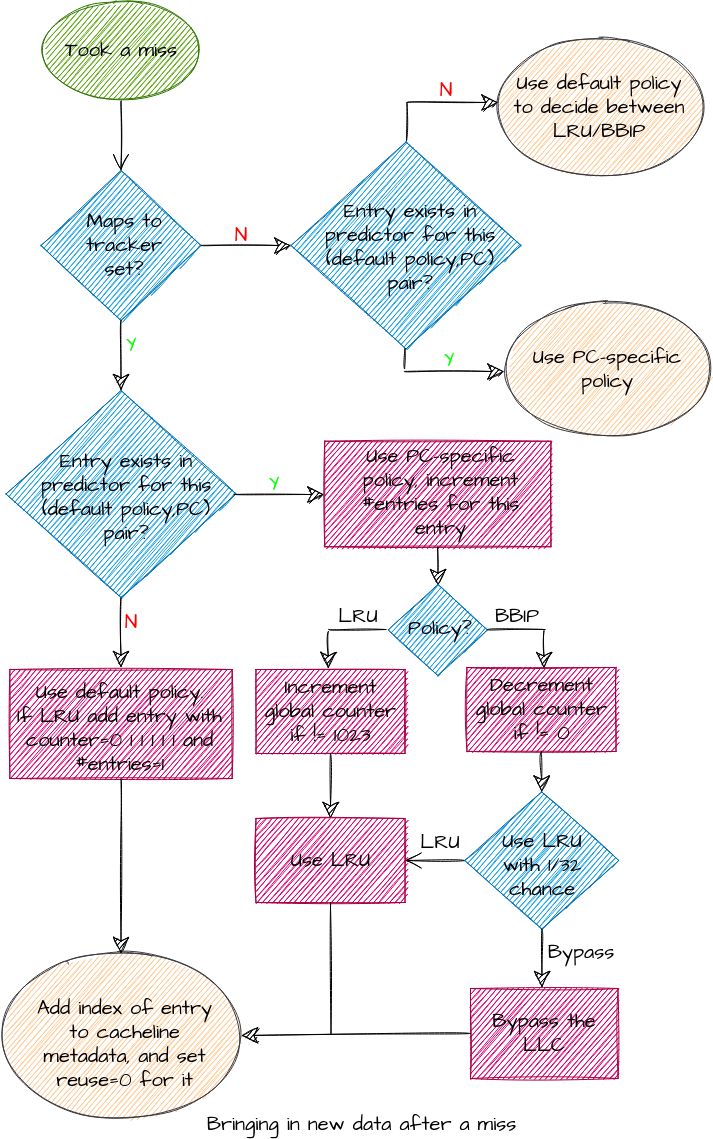
\includegraphics[width=0.6\linewidth]{images/newcacheline.png}
\end{figure}
If the \texttt{(Policy, PC)} pair exists in the predictor, we use the custom policy to decide what to do. This occurs even for lines not in tracker sets (we map those cachelines whose index bits have 0101 as the 4 LSBs as tracker sets; i.e., 1/16 of all cachelines are tracker sets). However, for these non-tracker lines, we do \textbf{not} create an entry in the predictor. However, if the cacheline \textit{is} part of a tracker set, we check to see if an entry exists in the predictor. If so, we use the corresponding custom policy and increment its \texttt{\#entries} field if it happens to be LRU (we shouldn't and don't do this for Bypass since there is no cacheline allocated in that case). Otherwise, we fall back to using the default policy and try to allocate a free predictor entry for this cacheline. If this succeeds, we initialize it with a counter of 011111 (``just'' LRU) and a \texttt{\#entries} field of 1. Note that if the allocation fails, we treat this cacheline just as if it were a non-tracker line henceforth (until new data is brought into it again).\\
If the policy used is LRU, we initialize the cacheline by setting \texttt{reuse=0} and the \texttt{pc\_pred\_index} to point to the allocated predictor entry. \\
Further, whenever we see a miss that maps to a tracker set, we check if we have a PC-specific policy for this PC. If so, we correspondingly change the global counter to penalize that specific type of behavior (since it caused us a miss). This implements set dueling (or ``PC dueling'', rather) between the LRU and Bypass sets.
We next look at the lifetime of a tracker cacheline in the LLC. Refer to the flowchart below.
\begin{figure}[H]
    \centering
    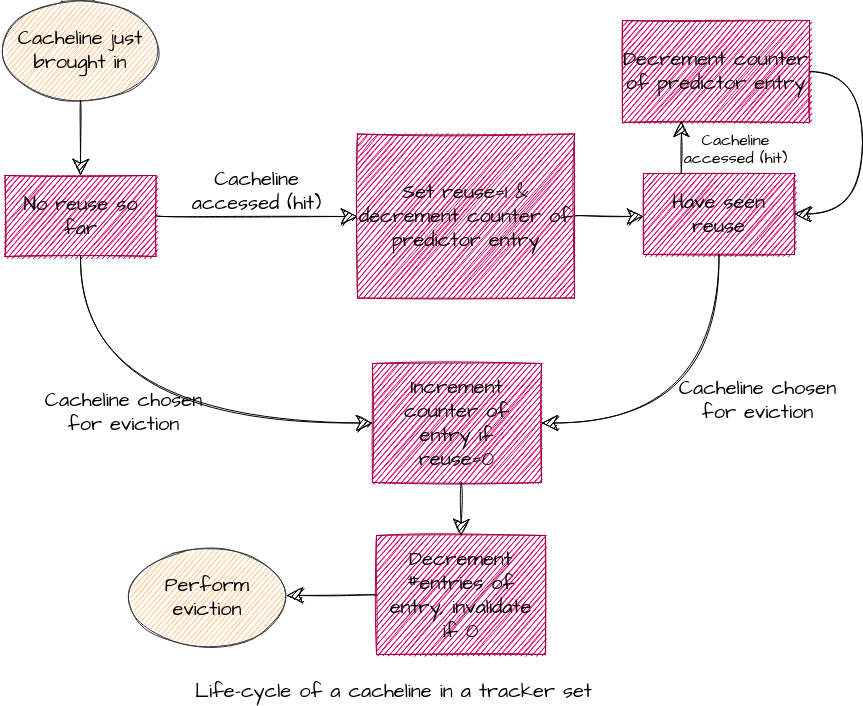
\includegraphics[width=0.85\linewidth]{images/lifecycle.png}
\end{figure}
A tracker cacheline starts with a \texttt{reuse} bit of 0 and a counter initialized to 31 (if it was the first one for that entry). Whenever this cacheline sees a hit, it means that we were right to use LRU; thus, we decrement the corresponding predictor entry's counter to make the behavior more ``LRU-like'' for this PC. We also set \texttt{reuse=1} for this cacheline on a hit. On the other hand, when the cacheline is being evicted, if we see a reuse bit of 0, this means that the cacheline was never used again; we should have bypassed the LLC. Thus we increment the corresponding counter. In either case, we decrement the \texttt{\#entries} field of the counter on eviction, and if it falls to 0, de-allocate the predictor entry (so that it can be used by future misses).

\section{Source files edited or added}
We modified the following files to implement the above scheme:
\begin{itemize}
    \item The files \texttt{inc/block.h} and \texttt{src/block.cc} contain the implementation of the predictor class.
    \item The file \texttt{inc/cache.h} has the definitions of a few helper functions and the modifications of the \texttt{CACHE} class to include the predictor.
    \item The file \texttt{src/cache.cc} contains the bulk of the changes, and implements the core logic of the above scheme. In particular, the functions that handle reads, writebacks and fills see extensive changes. Some other functions also see minor modifications.
\end{itemize}

\section{Impact on IPC}
The baseline LRU scheme gave an IPC of 0.142776 on average. On the other hand, our scheme gave an IPC of 0.171424 on average.\\
This corresponds to an increase (improvement) in IPC by roughly \textbf{20.065\%}.



%%%%%%%%%%%%%%%%%%%%%%%%%%%%%%%%%%%%%%%%%%%%%%%%
%% Prefetching
%%%%%%%%%%%%%%%%%%%%%%%%%%%%%%%%%%%%%%%%%%%%%%%%
\chapter{Prefetching}

\section{Implementation}
Each IP initially has the prefetch degree set to $3$. We dynamically update it based on the per-IP accuracy of the prefetches.\\
For each IP, we track the number of useful and useless prefetches. Whenever any prefetch is marked as useful or useless in \texttt{cache.cc}, the \texttt{prefetch\_throttle} function is called (depending on the cache type), and these values are updated for the respective IP. \texttt{prefetch\_throttle} updates the degree based on the throttle policy.

\subsection{Throttle Policy}
For a cache, we define $d_u, d_l$ as the upper and lower bounds on the prefetch degree and $t$ as the threshold. \\
For an IP, updates to the degree occur only after \texttt{prefetch\_throttle} is called $10$ times for that IP; this counter is reset after every update. \\
Updates happen based on the accuracy, which is the ratio of useful to useful $+$ useless prefetches. \\
If accuracy is $> t$, then the degree is incremented by $1$, unless it's already equal to $d_u$. \\
If accuracy is $\le t$, then the degree is decremented by $1$, unless it's already equal to $d_l$. \\
Sections \ref{section:ipc} \& \ref{section:ac} report the results for different values of $t$, for each cache, keeping $d_l, d_u$ fixed as: \\
L1D: $d_l = 1, d_u = 8$ \\
L2C: $d_l = 1, d_u = 16$

\subsection{Selecting $d_l, d_u$}
$d_l$ has been fixed to $1$ throughout; we don't tune this parameter. Figures \ref{fig:l1d}, \ref{fig:l2c} contain the results that help us choose $d_u$. Section \ref{sec:result_values} contains the respective numeric values obtained.\\
For L1D, we first fix the parameters for L2C at the baseline ($d_u = d_l = 3$, i.e., no throttling) then we compute the metrics for all combinations of $t \in \{0.25, 0.5, 0.75\}$ and $d_u \in \{4, 6, 8\}$. We observe that $d_u = 8$ gives the highest IPC. Thus, we set $d_u = 8$ for L1D.\\
For L2C, we first fix the parameters for L1D at the baseline ($d_u = d_l = 3$, i.e., no throttling) then we compute the results for all combinations of $t \in \{0.25, 0.5, 0.75\}$ and $d_u \in \{6, 8, 10, 12\}$. From these results, we observe that the results are poor for threshold values 0.5 and 0.75 and stay approximately the same. This could be since the accuracy values for IPs in L2C are low; they always tend to stay below $0.5$; thus, the degree quickly reduces to $1$ and stays $1$ throughout. This motivates us to change the set of $t$ values that we are considering. We also observe that for a fixed threshold, the best results are obtained for $d_u = 16$. Thus, we run more experiments for $d_u = 16$ and $t \in \{0.05, 0.15\}$. We observe that the best IPC is obtained for $t = 0.05$ and $d_u = 16$. Thus, we set $d_u = 16$ for L2C.

\medskip
Finally, after fixing $d_u, d_l$ for both the caches, we compute the results for all combinations of $t_{L1D} \in \{0.25, 0.5, 0.75\}$ and $t_{L2C} \in \{0.05, 0.15, 0.25\}$ and report these in sections \ref{section:ipc} and \ref{section:ac}.

\begin{figure}[H]
    \centering
    {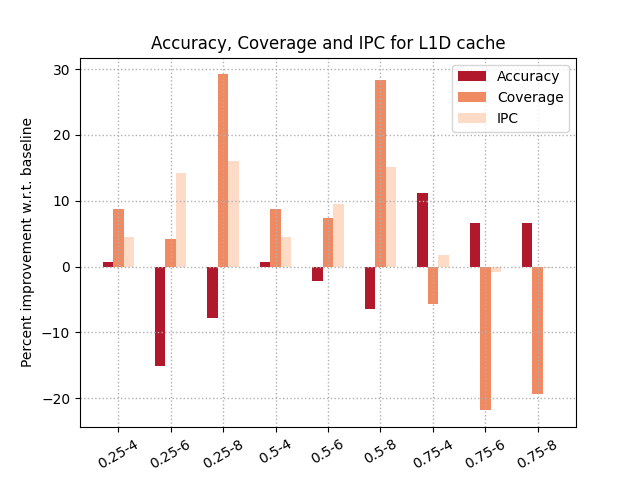
\includegraphics[scale = 0.65]{images/L1D.png}}
    \caption{Labels on the $x$-axis are of the form $t$--$d_u$}
    \label{fig:l1d}
\end{figure}

\begin{figure}[H]
    \centering
    {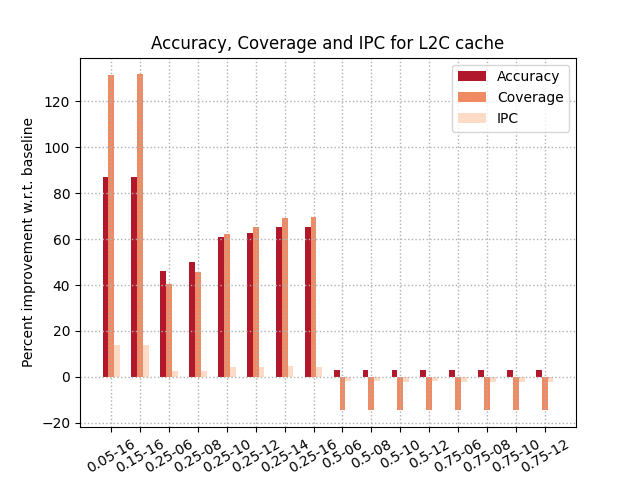
\includegraphics[scale = 0.65]{images/L2C.png}}
    \caption{Labels on the $x$-axis are of the form $t$--$d_u$}
    \label{fig:l2c}
\end{figure}

\section{Normalized IPC improvement wrt thresholds}
\label{section:ipc}

\begin{figure}[H]
    \centering
    {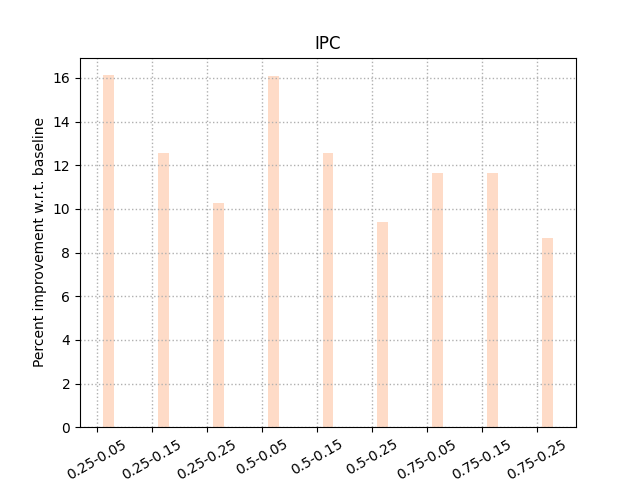
\includegraphics[scale = 1]{images/combined_ipcs.png}}
    \caption{Labels on the $x$-axis are of the form $t_{L1D}$--$t_{L2C}$}
    \label{fig:ipcs}
\end{figure}

\section{Prefetcher accuracies and coverage wrt thresholds}
\label{section:ac}

\begin{figure}[H]
    \centering
    {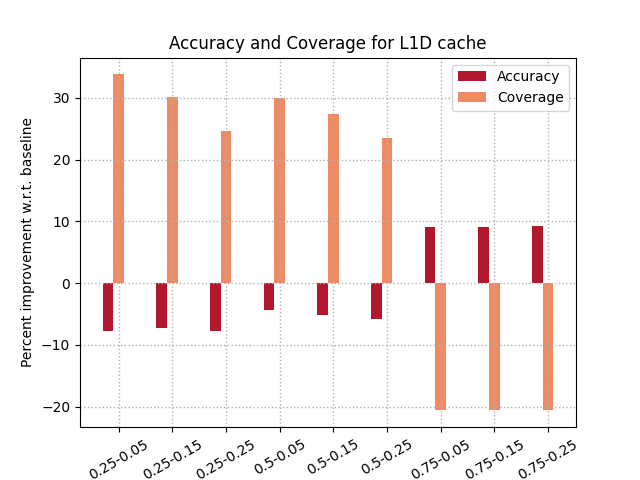
\includegraphics[scale = 0.7]{images/combined_L1D.png}}
    \caption{Labels on the $x$-axis are of the form $t_{L1D}$--$t_{L2C}$}
    \label{fig:cl1d}
\end{figure}

\begin{figure}[H]
    \centering
    {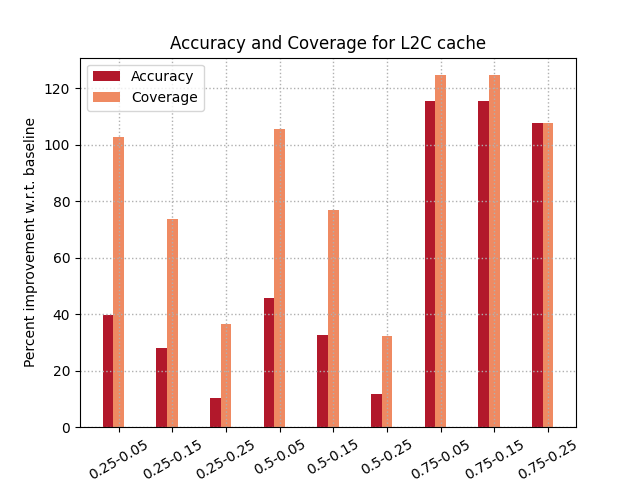
\includegraphics[scale = 0.7]{images/combined_L2C.png}}
    \caption{Labels on the $x$-axis are of the form $t_{L1D}$--$t_{L2C}$}
    \label{fig:cl2c}
\end{figure}

\section{Results (Values)}
\label{sec:result_values}

\begin{figure}[H]
    \centering
    \begin{BVerbatim}
----------------------L1D----------------------
+--------+------------+------------+----------+
| t-d_u  |   Accuracy |   Coverage |      IPC |
|--------+------------+------------+----------|
| 0.25-4 |   0.712436 |   0.269298 | 0.222645 |
| 0.25-6 |   0.600354 |   0.258107 | 0.243394 |
| 0.25-8 |   0.652155 |   0.319944 | 0.247193 |
| 0.5-4  |   0.712436 |   0.269298 | 0.222645 |
| 0.5-6  |   0.691499 |   0.265962 | 0.23328  |
| 0.5-8  |   0.661731 |   0.317649 | 0.24555  |
| 0.75-4 |   0.786124 |   0.233487 | 0.21702  |
| 0.75-6 |   0.754459 |   0.19353  | 0.211511 |
| 0.75-8 |   0.754403 |   0.199547 | 0.212759 |
+--------+------------+------------+----------+
    \end{BVerbatim}
    \caption{Results related to figure \ref{fig:l1d}}
\end{figure}

\begin{figure}[H]
    \centering
    \begin{BVerbatim}
----------------------L2C----------------------
+---------+------------+------------+----------+
| t-d_u   |   Accuracy |   Coverage |      IPC |
|---------+------------+------------+----------|
| 0.05-16 |   0.322317 |   0.364969 | 0.242624 |
| 0.15-16 |   0.322932 |   0.365557 | 0.242304 |
| 0.25-06 |   0.251878 |   0.221186 | 0.218375 |
| 0.25-08 |   0.258495 |   0.229774 | 0.218577 |
| 0.25-10 |   0.277876 |   0.256039 | 0.22223  |
| 0.25-12 |   0.280375 |   0.260855 | 0.22239  |
| 0.25-14 |   0.284907 |   0.267188 | 0.222789 |
| 0.25-16 |   0.285274 |   0.267735 | 0.222762 |
| 0.5-06  |   0.177547 |   0.13465  | 0.209062 |
| 0.5-08  |   0.177547 |   0.13465  | 0.209062 |
| 0.5-10  |   0.177679 |   0.134674 | 0.208561 |
| 0.5-12  |   0.177547 |   0.13465  | 0.209062 |
| 0.75-06 |   0.177679 |   0.134674 | 0.208561 |
| 0.75-08 |   0.177679 |   0.134674 | 0.208561 |
| 0.75-10 |   0.177679 |   0.134674 | 0.208561 |
| 0.75-12 |   0.177679 |   0.134674 | 0.208561 |
+---------+------------+------------+----------+
    \end{BVerbatim}
    \caption{Results related to figure \ref{fig:l2c}}
\end{figure}

\begin{figure}[H]
    \centering
    \begin{BVerbatim}
----------------------L1D----------------------
+-----------+------------+------------+----------+
| t_1d-t_2c |   Accuracy |   Coverage |      IPC |
|-----------+------------+------------+----------|
| 0.25-0.05 |   0.653101 |   0.331389 | 0.247562 |
| 0.25-0.15 |   0.655644 |   0.322231 | 0.23995  |
| 0.25-0.25 |   0.652448 |   0.308576 | 0.23507  |
| 0.5-0.05  |   0.676553 |   0.321961 | 0.247528 |
| 0.5-0.15  |   0.671388 |   0.315496 | 0.239972 |
| 0.5-0.25  |   0.666546 |   0.305828 | 0.233228 |
| 0.75-0.05 |   0.77162  |   0.196809 | 0.238049 |
| 0.75-0.15 |   0.77177  |   0.196702 | 0.237963 |
| 0.75-0.25 |   0.77263  |   0.196597 | 0.231663 |
+-----------+------------+------------+----------+
    \end{BVerbatim}
    \caption{Results related to figure \ref{fig:cl1d}}
\end{figure}

\begin{figure}[H]
    \centering
    \begin{BVerbatim}
----------------------L2C----------------------
+-----------+------------+------------+----------+
| t_1d-t_2c |   Accuracy |   Coverage |      IPC |
|-----------+------------+------------+----------|
| 0.25-0.05 |   0.241089 |   0.319648 | 0.247562 |
| 0.25-0.15 |   0.220957 |   0.27399  | 0.23995  |
| 0.25-0.25 |   0.190415 |   0.215303 | 0.23507  |
| 0.5-0.05  |   0.251362 |   0.324468 | 0.247528 |
| 0.5-0.15  |   0.228838 |   0.27902  | 0.239972 |
| 0.5-0.25  |   0.192552 |   0.208844 | 0.233228 |
| 0.75-0.05 |   0.371984 |   0.35425  | 0.238049 |
| 0.75-0.15 |   0.371986 |   0.354375 | 0.237963 |
| 0.75-0.25 |   0.358576 |   0.32765  | 0.231663 |
+-----------+------------+------------+----------+
    \end{BVerbatim}
    \caption{Results related to figure \ref{fig:cl2c}}
\end{figure}

\section{Source files edited or added}
\vspace{-0.8em}
\begin{verbatim}
Edited:
    ChampSim/inc/cache.h
    ChampSim/src/cache.cc
    ChampSim/prefetcher/ip_stride.l2c_pref
    ChampSim/prefetcher/no.l2c_pref
    ChampSim/prefetcher/no.l1d_pref
Added:
    ChampSim/inc/ip_stride.h
    ChampSim/prefetcher/ip_stride.l1d_pref
\end{verbatim}

\chapter{Running the code}
\section{Part 1: LLC Bypassing}
The decision variable used to decide whether to use the implemented version or the baseline is \texttt{LLC\_BYPASS} in \texttt{champsim.h} file. If it is defined, then the code will use Madcache; otherwise, it uses the default LRU policy.\\
The commands used are:
\begin{verbatim}
    ./build_champsim.sh bimodal no no no no lru 1
    ./run_champsim.sh bimodal-no-no-no-no-lru-1core 10 10 trace.champsimtrace.xz
\end{verbatim}
\section{Part 3: Prefetching}
Disable LLC Bypassing as explained above.(Comment out the line defining \texttt{LLC\_BYPASS} in \texttt{champsim.h}.) The prefetchers are defined in the files \texttt{ip\_stride.l2c\_pref} and \texttt{ip\_stride.l1d\_pref}. So, depending on which prefetcher to use, pass the name while running \texttt{build\_champsim.sh}.\\
The commands will be:
\begin{verbatim}
Only L1D prefetching:
    ./build_champsim.sh bimodal no ip_stride no no lru 1
    ./run_champsim.sh bimodal-no-ip_stride-no-no-lru-1core 10 10 trace.champsimtrace.xz
Only L2C prefetching:
    ./build_champsim.sh bimodal no no ip_stride no lru 1
    ./run_champsim.sh bimodal-no-no-ip_stride-no-lru-1core 10 10 trace.champsimtrace.xz
Combined:
    ./build_champsim.sh bimodal no ip_stride ip_stride no lru 1
    ./run_champsim.sh bimodal-no-ip_stride-ip_stride-no-lru-1core 10 10 trace.champsimtrace.xz
\end{verbatim}
The threshold and the bounds are defined in the respective file with the names \texttt{ACCURACY\_TH}, \texttt{DEGREE\_LOWER\_BOUND} and \texttt{DEGREE\_UPPER\_BOUND}. Set both \texttt{DEGREE\_LOWER\_BOUND} and \texttt{DEGREE\_UPPER\_BOUND} to $3$ to get the baseline result.



%%%%%%%%%%%%%%%%%%%%%%%%%%%%%%%%%%%%%%%%%%%%%%%%
%% Contributions
%%%%%%%%%%%%%%%%%%%%%%%%%%%%%%%%%%%%%%%%%%%%%%%%
\chapter{Contributions}
 {
  \renewcommand{\arraystretch}{1.2}  % For increased padding
  \begin{table}[h]
      \centering
      \begin{tabular}{|c|c|p{6cm}|}
          \hline
          \textbf{Member} & \textbf{Work Done}                                         \\
          \hline
          \hline
          Vibhav Aggarwal & Part 3 code and experiments, plotter scripts               \\
          Adithya Bhaskar & Part 1 code, part 2 explanation                            \\
          Devansh Jain    & Part 0 summary, part 1 code testing, result for part 2     \\
          Harshit Varma   & Part 3 code and experiments, part 4                        \\
          Harshit Gupta   & Part 0 code explanation, part 1 code testing, code merging \\
          \hline
      \end{tabular}
      \caption{Contributions of each team member}
  \end{table}
 }



\end{document}
